% Generated by extension/synthesis/make_assets.py. Do not edit.
\definecolor{propcol}{HTML}{217D91}
\definecolor{pairedcol}{HTML}{5D6670}
\definecolor{semicol}{HTML}{C9803A}
\definecolor{champcol}{HTML}{8E4B8C}
\definecolor{ridgecol}{HTML}{9AA3AB}
\definecolor{meancol}{HTML}{A64442}
\definecolor{sitecol}{HTML}{6A8FB3}
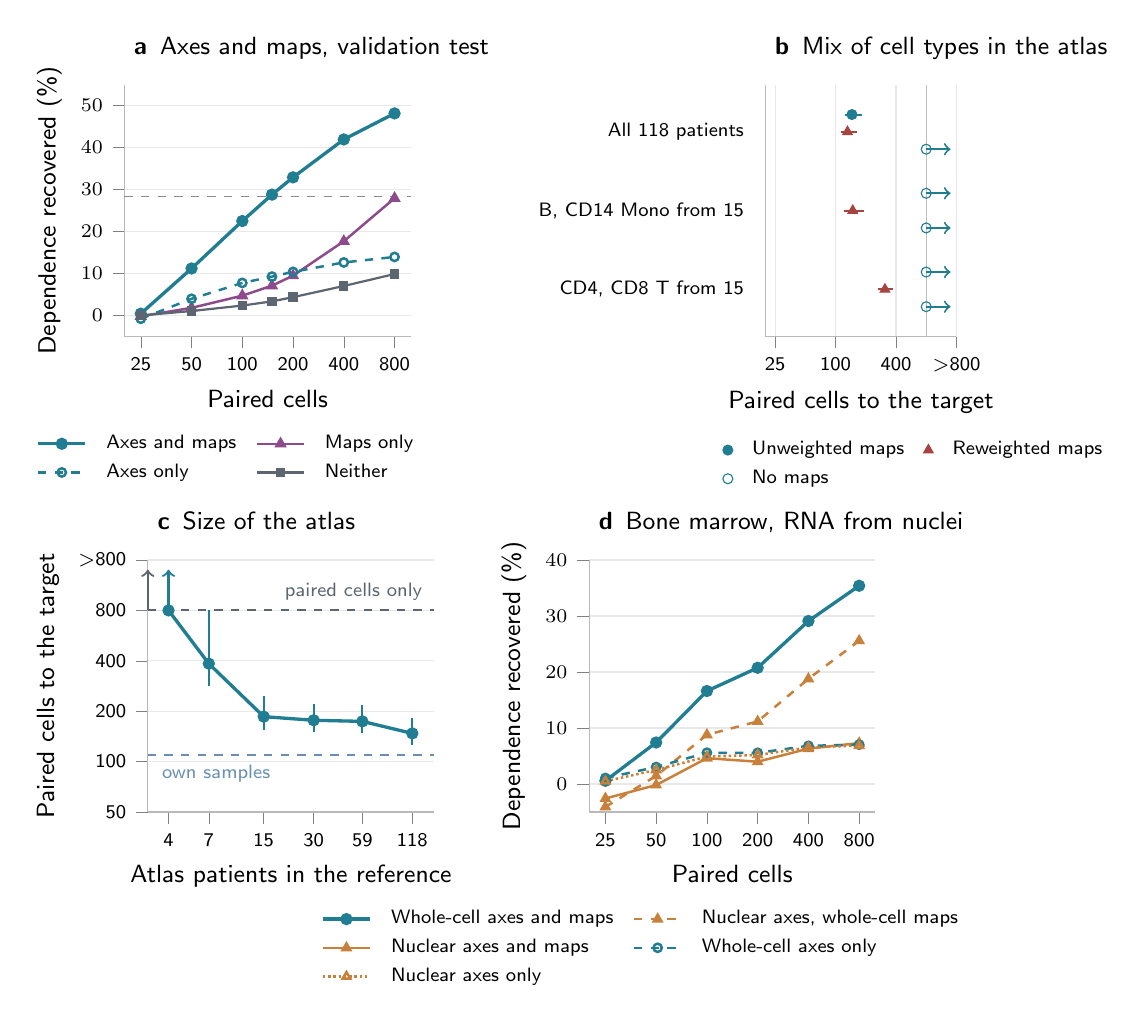
\begin{tikzpicture}[font=\sffamily]
\begin{axis}[name=a,scale only axis,width=.3\textwidth,height=3.2cm,xmode=log,log basis x=2,
 xmin=20,xmax=1000,ymin=-5,ymax=55,xtick={25,50,100,200,400,800},xticklabels={25,50,100,200,400,800},ytick={0,10,20,30,40,50},
 xlabel={Paired cells},ylabel={Dependence recovered (\%)},
 title={\textbf{a}\enspace Axes and maps, validation test},
 axis x line*=bottom,axis y line*=left,tick align=outside,ymajorgrids=true,grid style={gray!18},axis line style={gray!55},tick label style={font=\sffamily\scriptsize},label style={font=\sffamily\small},clip=false,title style={font=\sffamily\small,at={(0,1)},anchor=base west,yshift=5pt}]
\draw[dashed,black!45] (axis cs:20,28.34) -- (axis cs:1000,28.34);
\addplot[color=propcol,line width=1.2pt,mark=*,mark size=1.6pt] coordinates { (25,0.46) (50,11.22) (100,22.52) (150,28.81) (200,32.92) (400,41.95) (800,48.15) };
\addplot[color=champcol,line width=.9pt,mark=triangle*,mark size=1.7pt] coordinates { (25,-0.16) (50,1.84) (100,4.75) (150,7.12) (200,9.52) (400,17.70) (800,27.95) };
\addplot[color=propcol,line width=.9pt,dashed,mark=o,mark size=1.5pt,mark options={solid}] coordinates { (25,-0.75) (50,4.00) (100,7.78) (150,9.28) (200,10.42) (400,12.66) (800,13.97) };
\addplot[color=pairedcol,line width=.8pt,mark=square*,mark size=1.3pt] coordinates { (25,0.04) (50,1.09) (100,2.39) (150,3.39) (200,4.39) (400,7.05) (800,9.90) };
\end{axis}
\begin{axis}[at={(a.outer north east)},anchor=outer north west,xshift=.4cm,name=b,scale only axis,width=.2\textwidth,height=3.2cm,xmode=log,log basis x=2,
 xmin=20,xmax=1600,ymin=.4,ymax=3.6,xtick={25,100,400,1600},xticklabels={25,100,400,$>$800},
 ytick={1,2,3},
 yticklabels={{CD4, CD8 T from 15},{B, CD14 Mono from 15},{All 118 patients}},
 xlabel={Paired cells to the target},
 title={\textbf{b}\enspace Mix of cell types in the atlas},
 axis x line*=bottom,axis y line*=left,tick align=outside,xmajorgrids=true,grid style={gray!18},axis line style={gray!55},tick label style={font=\sffamily\scriptsize},label style={font=\sffamily\small},clip=false,title style={font=\sffamily\small,at={(0,1)},anchor=base west,yshift=5pt},y tick style={draw=none}]
\draw[black!25] (axis cs:800,.4) -- (axis cs:800,3.6);
\draw[->,color=propcol,line width=.7pt] (axis cs:800,1.22) -- (axis cs:1400,1.22);
\addplot[only marks,mark=o,mark size=1.8pt,color=propcol] coordinates { (800,1.22) };
\draw[color=meancol,line width=.7pt] (axis cs:266.4,1.00) -- (axis cs:377.6,1.00);
\addplot[only marks,mark=triangle*,mark size=2pt,color=meancol] coordinates { (310.5,1.00) };
\draw[->,color=propcol,line width=.7pt] (axis cs:800,0.78) -- (axis cs:1400,0.78);
\addplot[only marks,mark=o,mark size=1.8pt,color=propcol] coordinates { (800,0.78) };
\draw[->,color=propcol,line width=.7pt] (axis cs:800,2.22) -- (axis cs:1400,2.22);
\addplot[only marks,mark=o,mark size=1.8pt,color=propcol] coordinates { (800,2.22) };
\draw[color=meancol,line width=.7pt] (axis cs:122.4,2.00) -- (axis cs:191.6,2.00);
\addplot[only marks,mark=triangle*,mark size=2pt,color=meancol] coordinates { (148.2,2.00) };
\draw[->,color=propcol,line width=.7pt] (axis cs:800,1.78) -- (axis cs:1400,1.78);
\addplot[only marks,mark=o,mark size=1.8pt,color=propcol] coordinates { (800,1.78) };
\draw[color=propcol,line width=.7pt] (axis cs:123.5,3.22) -- (axis cs:183.5,3.22);
\addplot[only marks,mark=*,mark size=1.8pt,color=propcol] coordinates { (145.5,3.22) };
\draw[color=meancol,line width=.7pt] (axis cs:113.5,3.00) -- (axis cs:162.0,3.00);
\addplot[only marks,mark=triangle*,mark size=2pt,color=meancol] coordinates { (131.4,3.00) };
\draw[->,color=propcol,line width=.7pt] (axis cs:800,2.78) -- (axis cs:1400,2.78);
\addplot[only marks,mark=o,mark size=1.8pt,color=propcol] coordinates { (800,2.78) };
\end{axis}
\begin{axis}[hide axis,scale only axis,width=1pt,height=1pt,xmin=0,xmax=1,ymin=0,ymax=1,at={(a.outer south west)},anchor=north west,yshift=-2pt,legend style={draw=none,font=\sffamily\scriptsize,at={(0,0.5)},anchor=north west,legend columns=2,column sep=5pt,cells={anchor=west}}]
\addlegendimage{color=propcol,line width=1.2pt,mark=*,mark size=1.6pt}
\addlegendentry{Axes and maps}
\addlegendimage{color=champcol,line width=.9pt,mark=triangle*,mark size=1.7pt}
\addlegendentry{Maps only}
\addlegendimage{color=propcol,line width=.9pt,dashed,mark=o,mark size=1.5pt,mark options={solid}}
\addlegendentry{Axes only}
\addlegendimage{color=pairedcol,line width=.8pt,mark=square*,mark size=1.3pt}
\addlegendentry{Neither}
\end{axis}
\begin{axis}[hide axis,scale only axis,width=1pt,height=1pt,xmin=0,xmax=1,ymin=0,ymax=1,at={(b.outer south east)},anchor=north east,yshift=-2pt,legend style={draw=none,font=\sffamily\scriptsize,at={(1,0.5)},anchor=north east,legend columns=2,column sep=5pt,cells={anchor=west}}]
\addlegendimage{only marks,mark=*,mark size=1.8pt,color=propcol}
\addlegendentry{Unweighted maps}
\addlegendimage{only marks,mark=triangle*,mark size=2pt,color=meancol}
\addlegendentry{Reweighted maps}
\addlegendimage{only marks,mark=o,mark size=1.8pt,color=propcol}
\addlegendentry{No maps}
\end{axis}
\begin{axis}[at={(a.outer south west)},anchor=outer north west,yshift=-1.1cm,name=c,scale only axis,width=.3\textwidth,height=3.2cm,xmode=log,log basis x=2,
 ymode=log,log basis y=2,xmin=3,xmax=160,ymin=50,ymax=1600,xtick={4,7,15,30,59,118},xticklabels={4,7,15,30,59,118},
 ytick={50,100,200,400,800,1600},yticklabels={50,100,200,400,800,$>$800},
 xlabel={Atlas patients in the reference},ylabel={Paired cells to the target},
 title={\textbf{c}\enspace Size of the atlas},
 axis x line*=bottom,axis y line*=left,tick align=outside,ymajorgrids=true,grid style={gray!18},axis line style={gray!55},tick label style={font=\sffamily\scriptsize},label style={font=\sffamily\small},clip=false,title style={font=\sffamily\small,at={(0,1)},anchor=base west,yshift=5pt}]
\draw[color=pairedcol,line width=.8pt,->] (axis cs:3,800) -- (axis cs:3,1400);
\draw[color=pairedcol,dashed,line width=.7pt] (axis cs:3,800) -- (axis cs:160,800);
\draw[color=sitecol,dashed,line width=.7pt] (axis cs:3,109.6) -- (axis cs:160,109.6);
\node[font=\sffamily\scriptsize,color=pairedcol,anchor=south east] at (axis cs:155,800) {paired cells only};
\node[font=\sffamily\scriptsize,color=sitecol,anchor=north west] at (axis cs:3.2,109.6) {own samples};
\draw[->,color=propcol,line width=.8pt] (axis cs:4,800) -- (axis cs:4,1400);
\draw[color=propcol,line width=.8pt] (axis cs:7,281.0) -- (axis cs:7,800.0);
\draw[color=propcol,line width=.8pt] (axis cs:15,154.8) -- (axis cs:15,245.7);
\draw[color=propcol,line width=.8pt] (axis cs:30,150.7) -- (axis cs:30,219.4);
\draw[color=propcol,line width=.8pt] (axis cs:59,147.3) -- (axis cs:59,217.3);
\draw[color=propcol,line width=.8pt] (axis cs:118,126.0) -- (axis cs:118,182.1);
\addplot[color=propcol,line width=1.2pt,mark=*,mark size=1.6pt] coordinates {(4,800.0) (7,384.6) (15,185.5) (30,176.5) (59,173.8) (118,147.3)};
\addplot[only marks,mark=o,mark size=1.8pt,color=propcol,fill=white] coordinates { (4,800) };
\end{axis}
\begin{axis}[at={(c.outer north east)},anchor=outer north west,xshift=.4cm,name=d,scale only axis,width=.3\textwidth,height=3.2cm,xmode=log,log basis x=2,
 xmin=20,xmax=1000,ymin=-5,ymax=40,xtick={25,50,100,200,400,800},xticklabels={25,50,100,200,400,800},ytick={0,10,20,30,40},
 xlabel={Paired cells},ylabel={Dependence recovered (\%)},
 title={\textbf{d}\enspace Bone marrow, RNA from nuclei},
 axis x line*=bottom,axis y line*=left,tick align=outside,ymajorgrids=true,grid style={gray!18},axis line style={gray!55},tick label style={font=\sffamily\scriptsize},label style={font=\sffamily\small},clip=false,title style={font=\sffamily\small,at={(0,1)},anchor=base west,yshift=5pt}]
\addplot[color=propcol,line width=1.2pt,mark=*,mark size=1.6pt] coordinates { (25,0.57) (50,7.41) (100,16.60) (200,20.75) (400,29.10) (800,35.40) };
\addplot[color=semicol,line width=.9pt,dashed,mark=triangle*,mark size=1.6pt,mark options={solid}] coordinates { (25,-4.10) (50,1.45) (100,8.78) (200,11.17) (400,18.77) (800,25.58) };
\addplot[color=semicol,line width=.9pt,mark=triangle*,mark size=1.6pt] coordinates { (25,-2.59) (50,-0.19) (100,4.61) (200,3.97) (400,6.32) (800,7.30) };
\addplot[color=propcol,line width=.9pt,dashed,mark=o,mark size=1.5pt,mark options={solid}] coordinates { (25,1.06) (50,3.02) (100,5.58) (200,5.56) (400,6.81) (800,7.03) };
\addplot[color=semicol,line width=.9pt,densely dotted,mark=triangle,mark size=1.6pt,mark options={solid}] coordinates { (25,0.49) (50,2.50) (100,4.89) (200,5.17) (400,6.53) (800,6.86) };
\end{axis}
\begin{axis}[hide axis,scale only axis,width=1pt,height=1pt,xmin=0,xmax=1,ymin=0,ymax=1,at={(d.outer south east)},anchor=north east,yshift=-2pt,legend style={draw=none,font=\sffamily\scriptsize,at={(1,0.5)},anchor=north east,legend columns=2,column sep=5pt,cells={anchor=west}}]
\addlegendimage{color=propcol,line width=1.2pt,mark=*,mark size=1.6pt}
\addlegendentry{Whole-cell axes and maps}
\addlegendimage{color=semicol,line width=.9pt,dashed,mark=triangle*,mark size=1.6pt,mark options={solid}}
\addlegendentry{Nuclear axes, whole-cell maps}
\addlegendimage{color=semicol,line width=.9pt,mark=triangle*,mark size=1.6pt}
\addlegendentry{Nuclear axes and maps}
\addlegendimage{color=propcol,line width=.9pt,dashed,mark=o,mark size=1.5pt,mark options={solid}}
\addlegendentry{Whole-cell axes only}
\addlegendimage{color=semicol,line width=.9pt,densely dotted,mark=triangle,mark size=1.6pt,mark options={solid}}
\addlegendentry{Nuclear axes only}
\end{axis}
\end{tikzpicture}
